\documentclass[handout, 11pt]{beamer}
\mode
<presentation>{\usetheme{Madrid}}
\institute[UF]{\inst{1}
University of Florida\\
Department of Finance, Insurance, and Real Estate}
\definecolor{darkgreen}{RGB}{31,156,17}
\usepackage{booktabs}
\usepackage{xcolor}
\setbeamertemplate{headline}{\begin{beamercolorbox}[ht=2.25ex, dp=3.75ex]{section in head/foot}
\insertnavigation{\paperwidth}
\end{beamercolorbox}}
\AtBeginSection{\begin{frame}
\frametitle{Table of Contents}
\tableofcontents[currentsection]
\end{frame}}
\begin{document}
\title[FCF]{Free Cash Flow Estimation and Forecasting}
\subtitle{Calculation and Projection}
\author[DeRobertis]{Nick DeRobertis\inst{1}}
\date{\today}
\begin{frame}
\titlepage
\label{title-frame}
\end{frame}
\begin{section}{Overview}
\begin{frame}
\frametitle{FCF Overview}
\begin{itemize}
\item There are two main parts to the FCF part of the DCF model
\vfill
\item First is to find all the historical FCFs. This is the straightforward part of plugging values into set calculations.
\vfill
\item The more difficult and important part is projecting future cash flows
\vfill
\item We will discuss a variety of approaches for this
\end{itemize}
\end{frame}
\begin{frame}
\frametitle{What is FCF?}
\begin{itemize}
\item Free cash flow (FCF) represents cash a company earns after paying for its operations.
\vfill
\item It is not to be confused with net income, which amortizes costs across years and includes non-cash expenses
\vfill
\item FCF represents only the cash flows from that year, and so can be a lot more variable than net income
\vfill
\item FCF is the actual cash earned, and so it is what we should use for valuation
\end{itemize}
\end{frame}
\begin{frame}
\frametitle{Historical FCFs}
\begin{columns}
\begin{column}{0.5\textwidth}
\vbox to 0.8\textheight{\begin{itemize}
\item We can follow a simple formula to get FCFs from historical financials
\vfill
\item All we have to do is calculate the formula for each year of historical data
\vfill
\item Each of the components to this calculation besides net income themselves require a calculation. In the Historical FCF section we will cover each component.
\vfill
\item The formula is all about reversing the non-cash adjustments to net income
\end{itemize}}
\end{column}
\begin{column}{0.5\textwidth}
\vbox to 0.8\textheight{\centering
\vfill
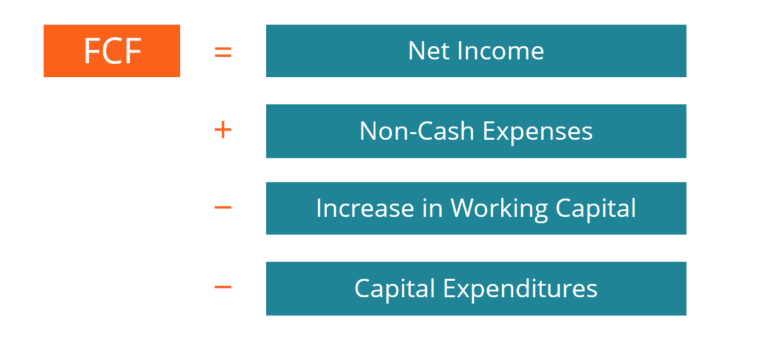
\includegraphics[height=1.0\textheight, keepaspectratio, width=0.9\textwidth]{Sources/fcf-formula.png}
\vfill
\vfill}
\end{column}
\end{columns}
\end{frame}
\begin{frame}
\frametitle{Forecasting FCFs}
\begin{itemize}
\item The challenge in the FCF model is to project the cash flows
\vfill
\item There are two main approaches to getting future FCFs:
\underline{forecast the FCFs}
and
\underline{forecast the financial statements.}
\vfill
\item Forecasting FCFs is much easier but is not as accurate, both due to lack of granularity and due to typically uneven FCFs
\vfill
\item We will use
\underline{time-series methods}
to forecast the financial statements, either in the
\underline{levels}
of the item, the
\underline{growth}
of the item, or as a
\underline{percentage of another item}
\end{itemize}
\end{frame}
\end{section}
\begin{section}[Historical FCF]{Calculating Historical Free Cash Flows}
\begin{frame}
\frametitle{Non-Cash Expenses}
\begin{block}{Calculate Non-Cash Expenses}
$\text{Adjustments} = \text{depreciation} + \text{amortization} + \text{stock-based compensation} + \text{impairment charges} + \text{gains/losses on investments}$
\end{block}
\vfill
\begin{itemize}
\item Non-cash expenses is just the sum of all items on the income statement that do not affect cash.
\vfill
\item This includes depreciation, amortization, stock-based compensation, impairment charges, and gains/losses on investments
\end{itemize}
\end{frame}
\begin{frame}
\frametitle{Change in Net Working Capital}
\begin{block}{Calculate Change in NWC}
\begin{equation}
	\Delta\text{NWC} = \text{NWC}_t - \text{NWC}_{t-1}
\end{equation}
\begin{equation}
	\text{NWC} = \text{Accounts Receivable} + \text{Inventory} - \text{Accounts Payable}
\end{equation}
\end{block}
\vfill
\begin{itemize}
\item Net Working Capital (NWC) represents cash actively tied up in daily transactions
\vfill
\item Cacluating the change in NWC requires information from this period as well as last period.
\vfill
\item First, calculate the NWC in each period using accounts receivable, inventory, and accounts payable.
\vfill
\item Then, take the difference between this period's NWC and last to get the change
\end{itemize}
\end{frame}
\begin{frame}
\frametitle{Capital Expenditures}
\begin{block}{Calculate CapEx}
\begin{equation}
	\text{CapEx} = \Delta\text{PPE} + \text{Depreciation \& Amortization}
\end{equation}
\end{block}
\vfill
\begin{itemize}
\item Capital Expenditures (CapEx) are outlays for fixed assets which get used over time, such as buildings or machinery.
\vfill
\item The change in Property, Plant and Equipment from the balance sheet can be used to estimate CapEx.
\vfill
\item Then you just need to add back the current depreciation \& amortization, as they decreased PPE even though no cash exchanged hands
\end{itemize}
\end{frame}
\begin{frame}
\frametitle{Put it All Together}
\begin{block}{Calculating FCF}
\begin{equation}
	\text{FCF} = \text{Net Income} + \text{Non-Cash Expenses} - \Delta\text{NWC} - \text{CapEx}
\end{equation}
\end{block}
\vfill
\begin{itemize}
\item Again, the FCF formula takes net income and reverses the non-cash adjustments
\vfill
\item Add back the non-cash expenses because no actual cash was spent
\vfill
\item Decrease by the change in NWC as an increase means additional cash was used for operations
\vfill
\item Decrease by CapEx because this cash was spent for a new building, machinery, etc.
\end{itemize}
\end{frame}
\begin{frame}
\frametitle{Example for Calculating FCFs}
{
\setbeamercolor{block title}{bg=darkgreen}
\begin{block}{Two Ways to Calculate FCFs in Python}
\begin{itemize}
\item Go to the course site and download the files in Historical FCF
\item There should be a Jupyter notebook as well as a data file
\item We will go through a couple approaches to calculating FCFs in Python.
\end{itemize}
\end{block}
}
\end{frame}
\begin{frame}
\frametitle{Calculate FCF Lab, Level 1}
{
\setbeamercolor{block title}{bg=violet}
\begin{block}{Free Cash Flow Calculation, Level 1}
\begin{enumerate}
\item Calculate free cash flow from the following information:
\item Net income is 300, the total of non-cash expenditures is 100, the changes in accounts receivable, inventory, accounts payable, and PPE are 1000, 500, 800, and 2000, and depreciation \& amortization is 200.
\end{enumerate}
\vfill
\begin{tabular*}{\textwidth}{@{\extracolsep{\fill}}ccccc}
\toprule
\hfill & Level 2: Slide \textcolor{blue}{\underline{\ref{labs:calculate-fcf-lab-2}}} & Answers 1: Slide \textcolor{blue}{\underline{\ref{labs:calculate-fcf-lab-1-answers}}} & Resources: Slide \textcolor{blue}{\underline{\ref{labs:calculate-fcf-lab-1-resources}}} & \hfill\\

\end{tabular*}
\end{block}
}
\label{labs:calculate-fcf-lab-1}
\end{frame}
\end{section}
\begin{section}[Forecasting Overview]{Approaches to Forecasting}
\begin{frame}
\frametitle{Overview of the Methods}
\begin{itemize}
\small
\vfill
\item As mentioned in the intro, we will use time-series methods on the levels of the item, the growth of the item, or as a percentage of another item
\vfill
\item Time-series methods are about numerically estimating future values based on past values
\vfill
\item Levels mean we forecast the numbers of the item itself, e.g. sales was 1M two years ago and 1.5M last year so we feed those numbers into our time-series model and predict 2M for the next year
\vfill
\item Growth means to first calculate the historical growth rate of the item, then forecast that. E.g. sales grew 10\% two years ago and 8\% last year so we expect it to grow 6\% this year
\vfill
\item Percentage of item methods link an item to another item. E.g. setting cost of goods sold to 60\% of sales. That percentage still needs to be forecasted
\vfill
\item Any forecast can be adjusted by the analyst's qualitative projections of the future. The forecast method may also have to be chosen with the qualitative analysis in mind
\end{itemize}
\end{frame}
\begin{frame}
\frametitle{What Are Time-Series Methods?}
\begin{columns}
\begin{column}{0.5\textwidth}
\vbox to 0.8\textheight{\begin{itemize}
\item Time-series methods seek to predict the future using the past
\vfill
\item There is a large variety of possible time-series models to use for forecasting
\vfill
\item They each use different characteristics of the past to assist in predicting the future
\end{itemize}}
\end{column}
\begin{column}{0.5\textwidth}
\vbox to 0.8\textheight{\centering
\vfill
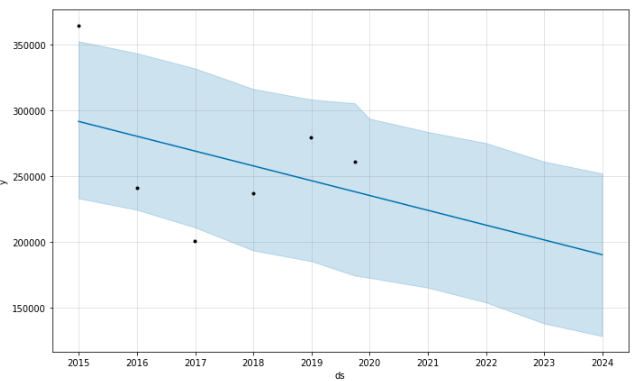
\includegraphics[height=1.0\textheight, keepaspectratio, width=0.9\textwidth]{Sources/time-series-linear-plot.png}
\vfill
\vfill}
\end{column}
\end{columns}
\end{frame}
\begin{frame}
\frametitle{What are the Time-Series Models?}
\begin{itemize}
\item The simplest models are to use the
\underline{average of historical values}
or the
\underline{most recent value}
as the prediction for all future values
\vfill
\item A more realistic model will also include estimating the
\underline{trend}
or \underline{growth} of the historical values and applying that to the future
\vfill
\item More advanced models use autoregressive terms (recent values predict future values), moving average terms (recent errors predict future values), or conditional heteroskedasticity terms (changing variance over time)
\vfill
\item Examples of these advanced models include AR, MA, ARMA, ARCH, GAM, and many more
\end{itemize}
\end{frame}
\begin{frame}
\frametitle{Which Time-Series Model to Use?}
\begin{itemize}
\item The choice of a time-series model will depend on the amount of data, the frequency of the data, and the historical patterns in the data
\vfill
\item If the data is historically constant or expected to be constant in the future, using the average or most recent value should be enough
\vfill
\item If the data follows a defined trend or growth and doesn't have historical patterns, then using the trend or growth models should be enough
\vfill
\item If there are historical patterns in the data, such as seasonality, then more advanced models are required.
\end{itemize}
\end{frame}
\begin{frame}
\frametitle{Steps to Forecasting}
\begin{itemize}
\item The best place to start is to
\underline{examine the history}
either by a plot
or just by looking at the numbers if you only have a few
\vfill
\item Based on the amount of historical data, any perceived patterns in the historical data, and any qualitative knowledge of the data,
\underline{choose a time-series model.}
\vfill
\item \underline{Fit}
the time-series model on historical data, then
\underline{predict}
the future values using the fitted model
\vfill
\item Finish by
\underline{examining the forecast}
to ensure it worked as intended, 
typically via a plot.
\end{itemize}
\end{frame}
\begin{frame}
\frametitle{What to Forecast?}
\begin{itemize}
\item When we forecast levels, just use the forecasted values and you are done
\vfill
\item When we forecast growth, calculate the historical growth, run the forecast on that, then apply the predicted future growth from the final historical period to generate the forecasted levels
\vfill
\item For percentage of item methods, calculate the historical percentage of the item, forecast future item percentages, then use these in combination with the forecast of the referenced item to generate the prediction
\vfill
\item E.g. use the average approach to say historically COGS was 40\% of sales, and so estimate COGS as 40\% of sales going forward. Multiply the forecasted sales by 40\% to get the COGS
\end{itemize}
\end{frame}
\end{section}
\begin{section}[Simple Forecast]{Forecasting Simple Time-Series}
\begin{frame}
\frametitle{Using the Historical Average Model}
\begin{block}{Historical Average Model}
\begin{equation}
	y_{T + n} = \frac{1}{T} \sum_{t=0}^T y_t + \epsilon_t
\end{equation}
\vspace{-0.3cm}
\begin{itemize}
\item $t$: Current time period
\item $T$: Last time period of historical data
\item $y_t$: The current value of the data
\item $y_T$: The last historical value of the data
\item $n$: Number of periods forecasted
\end{itemize}
\end{block}
\vfill
\begin{itemize}
\item \textbf{Fit:}
To fit the historical average model, take an average of the historical values
\vfill
\item \textbf{Predict:}
To predict, use that average value for all future values
\end{itemize}
\end{frame}
\begin{frame}
\frametitle{Using the Recent Value Model}
\begin{block}{Recent Value Model}
\begin{equation}
	y_t = y_{t-1} + \epsilon_t
\end{equation}
\end{block}
\vfill
\begin{itemize}
\item \textbf{Fit:}
To fit the most recent value model, take the latest value.
\vfill
\item \textbf{Predict:}
To predict, use that latest value for all future values
\end{itemize}
\end{frame}
\begin{frame}
\frametitle{Using the Trend Model}
\begin{block}{Trend Model}
\begin{equation}
	y_t = a + \beta t + \epsilon_t
\end{equation}
\end{block}
\vfill
\begin{itemize}
\item \textbf{Fit:}
Run an OLS regression with a constant and time as the independent variable, where time is measured in number of periods since the beginning
\vfill
\item \textbf{Predict:}
For each $t$ you want to predict, calculate $a + \beta t$
\end{itemize}
\end{frame}
\begin{frame}
\frametitle{Using the CAGR Model}
\begin{block}{CAGR}
\begin{equation}
	y_{{T + f}} = y_T * (\frac{y_T}{y_0}^{\frac{1}{n}})^f
\end{equation}
\end{block}
\vfill
\begin{itemize}
\item \textbf{Fit:}
Calculate the compounded annual growth rate (CAGR) as
$\frac{y_T}{y_0}^{\frac{1}{n}} - 1$
\vfill
\item \textbf{Predict:}
Calculate future periods by compounding CAGR on the latest historical period
$y_{T + f} = y_T * (1 + \text{CAGR})^f$
\end{itemize}
\end{frame}
\begin{frame}
\frametitle{Forecasting Simple Time-Series in both Excel and Python}
{
\setbeamercolor{block title}{bg=darkgreen}
\begin{block}{Example for Simple Time-Series Forecasting}
\begin{itemize}
\item Go to the course site and download the files in Examples > DCF > Forecasting > Simple
\item There should be a Jupyter notebook as well as two Excel files. Place these all in the same folder
\item We will walk through "Sales COGS Forecasted.xlsx" to show forecasting in Excel, and "Forecast Sales COGS Simple.ipynb" for forecasting in Python. "Sales COGS.xlsx" contains the source data
\end{itemize}
\end{block}
}
\end{frame}
\begin{frame}
\frametitle{Simple Forecast Lab}
{
\setbeamercolor{block title}{bg=violet}
\begin{block}{Forecasting Simple Time-Series}
\begin{enumerate}
\item Go to
\textcolor{blue}{\underline{\href{https://nickderobertis.github.io/fin-model-course/}{the course site}}}
and download "Debt Interest.xlsx"
\item Forecast the next value of total debt using trend regression approach
\item Forecast the next value of interest using the four approaches (average, recent, trend, CAGR)
\item Forecast the next value of interest using the \% of total debt method, with the percentages forecasted using the four approaches (average, recent, trend, CAGR)
\end{enumerate}
\vfill
\begin{tabular*}{\textwidth}{@{\extracolsep{\fill}}cccc}
\toprule
\hfill & Answers: Slide \textcolor{blue}{\underline{\ref{labs:simple-forecast-lab-1-answers}}} & Resources: Slide \textcolor{blue}{\underline{\ref{labs:simple-forecast-lab-1-resources}}} & \hfill\\

\end{tabular*}
\end{block}
}
\label{labs:simple-forecast-lab-1}
\end{frame}
\begin{frame}
\frametitle{Forecasting Financial Statements with Simple Time-Series in Python}
{
\setbeamercolor{block title}{bg=darkgreen}
\begin{block}{Use finstmt for Financial Statement Forecasting}
\begin{itemize}
\item Go to the course site and download "Forecasting Financial Statements.ipynb"
\item We will walk through using \texttt{finstmt} to forecast financial statements using simple time-series models
\end{itemize}
\end{block}
}
\end{frame}
\end{section}
\begin{section}[Complex Forecast]{Forecasting Complex Time-Series}
\begin{frame}
\frametitle{Why Does it get so Complicated?}
\begin{columns}
\begin{column}{0.5\textwidth}
\vbox to 0.8\textheight{\centering
\vfill
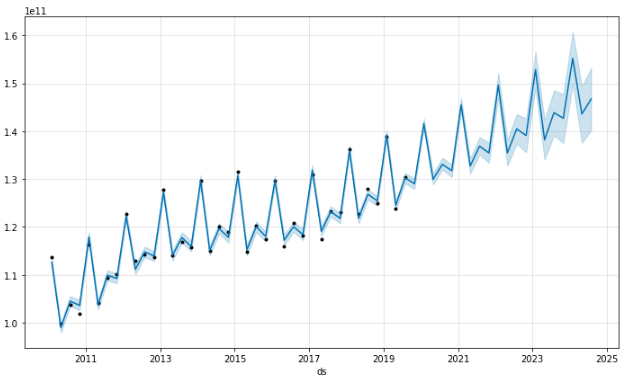
\includegraphics[height=1.0\textheight, keepaspectratio, width=0.9\textwidth]{Sources/time-series-plot.png}
\vfill
\vfill}
\end{column}
\begin{column}{0.5\textwidth}
\vbox to 0.8\textheight{\begin{itemize}
\item Shown to the left is Walmart's quarterly sales
\vfill
\item You can see that a plain trend line is never going to accurately forecast these values
\vfill
\item Advanced time-series models can capture these characteristics easily, and many more patterns
\end{itemize}}
\end{column}
\end{columns}
\end{frame}
\begin{frame}
\frametitle{Explaining Seasonal Data}
\begin{columns}
\begin{column}{0.5\textwidth}
\vbox to 0.8\textheight{\begin{itemize}
\item There is a distinct
\textbf{seasonality}
to Walmart's quarterly sales
\vfill
\item The time-series model used to create the plot on the prior slide split the history into two parts: a trend component and an annual seasonality component
\vfill
\item Walmart's sales are high at the end of January and neutral for the other quarters
\vfill
\item By plotting components of the time-series model, the analyst can gain a greater understanding of the business.
\end{itemize}}
\end{column}
\begin{column}{0.5\textwidth}
\vbox to 0.8\textheight{\centering
\vfill
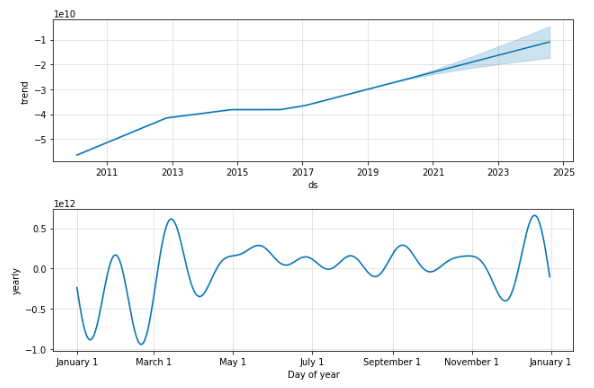
\includegraphics[height=1.0\textheight, keepaspectratio, width=0.9\textwidth]{Sources/time-series-plot-components.png}
\vfill
\vfill}
\end{column}
\end{columns}
\end{frame}
\begin{frame}
\frametitle{Predicting Complex Time-Series}
\begin{itemize}
\item So you've determined a trend alone will not fit the historical data. What are next steps?
\vfill
\item Generally fitting the best time-series model is an involved process which requires substantial knowledge of how the models work, see
\textcolor{blue}{\underline{\href{https://www.seanabu.com/2016/03/22/time-series-seasonal-ARIMA-model-in-python/}{this blog post}}}
for details
\vfill
\item An easier version is to use an OLS regression model with time and dummy variables for month of year, etc., we can call this the 
\underline{quarterly seasonal trend model.}
\vfill
\item The easiest version is to let time-series software, such as
\textcolor{blue}{\underline{\href{https://facebook.github.io/prophet/docs/quick\_start.html}{prophet}}}
make the choice for you
\end{itemize}
\end{frame}
\begin{frame}
\frametitle{Using the Quarterly Seasonal Trend Model}
\begin{block}{Quarterly Seasonal Trend Model}
\begin{equation}
	y_t = a + \beta_t t + \beta_{d1} D1 + \beta_{d2} D2 + \beta_{d3} D3 + \beta_{d4} D4  + \epsilon_t
\end{equation}
\end{block}
\vfill
\begin{itemize}
\item \textbf{Fit:}
Create dummy variables for the quarters, then run an OLS regression with the number of time periods as well as the four dummy variables as the $X$ variables
\vfill
\item \textbf{Predict:}
For each $t$ you want to predict, calculate $a + \beta t$ adding the appropriate dummy for the quarter of the period.
\end{itemize}
\end{frame}
\begin{frame}
\frametitle{Forecasting Complex Time-Series in Python}
{
\setbeamercolor{block title}{bg=darkgreen}
\begin{block}{Example for Complex Time-Series Forecasting}
\begin{itemize}
\item Go to the course site and download the files in Examples > DCF > Forecasting > Complex
\item There should be a Jupyter notebook as well as two Excel files. Place these all in the same folder
\item We will walk through "Forecasting Quarterly Financial Statements.ipynb" to show forecasting in Python using both the Quarterly Seasonal Trend Model and the automated software approach.
\end{itemize}
\end{block}
}
\end{frame}
\begin{frame}
\frametitle{Complex Forecast Lab}
{
\setbeamercolor{block title}{bg=violet}
\begin{block}{Forecasting Complex Time-Series}
\begin{enumerate}
\item Go to
\textcolor{blue}{\underline{\href{https://nickderobertis.github.io/fin-model-course/}{the course site}}}
and download "CAT Balance Sheet.xlsx" and "CAT Income Statement.xlsx"
\item Forecast the next four periods (one year) of cash using both the Quarterly Seasonal Trend Model and the automated software approach.
\item Plot both forecasts to see how they worked.
\end{enumerate}
\vfill
\begin{tabular*}{\textwidth}{@{\extracolsep{\fill}}cccc}
\toprule
\hfill & Answers: Slide \textcolor{blue}{\underline{\ref{labs:complex-forecast-lab-1-answers}}} & Resources: Slide \textcolor{blue}{\underline{\ref{labs:complex-forecast-lab-1-resources}}} & \hfill\\

\end{tabular*}
\end{block}
}
\label{labs:complex-forecast-lab-1}
\end{frame}
\end{section}
\begin{section}[Future FCFs]{Forecasting Free Cash Flows}
\begin{frame}
\frametitle{What to Forecast?}
\begin{itemize}
\item As mentioned in the intro, we can either directly forecast FCFs, or forecast the financial statements, then calculate future FCFs from the future financial statements
\vfill
\item Forecasting FCFs doesn't allow the analyst control over individual line items. Therefore it is generally preferred to forecast financial statements.
\vfill
\item If you have a short amount of time to put together the model, it can make sense as it is less steps and it requires less knowledge of the company.
\vfill
\item It can also make sense to do a FCF forecast alongside the financial statement forecast, as a check on your valuation.
\end{itemize}
\end{frame}
\begin{frame}
\frametitle{Which Line Items to Forecast?}
\begin{itemize}
\item Assuming you are going with forecasting financial statements, you should forecast only line items which cannot be calculated from other line items
\vfill
\item For example, sales, COGS, SG\&A should be forecasted, not operating profit
\vfill
\item You should set your model up so that these calculatable items are calculated in the historicals, then carry that through to the forecasted
\end{itemize}
\end{frame}
\end{section}
\begin{section}[Valuation]{Using the Forecasted FCFs in the DCF Model}
\begin{frame}
\frametitle{What we use FCFs For}
\begin{itemize}
\item As mentioned in the intro to the DCF model, we can value any asset by taking the present value of future cash flows
\vfill
\item These forecasted FCFs represent the future cash flows for the company
\vfill
\item But we have a limited forecast period, beyond which forecasts are getting too innaccurate, typically 5 years at most. So what happens after 5 years? The company will probably still be earning FCFs in the future.
\vfill
\item We can calculate a
\textbf{terminal value}
for the company, which is an estimate of how much the company would be sold for if it was sold at the end of the forecast period. In other words, it is the future predicted enterprise value.
\end{itemize}
\end{frame}
\begin{frame}
\frametitle{How to Get the Terminal Value}
\begin{itemize}
\item The terminal value is an enterprise value at the end of the forecast period. But the bulk of the DCF model is getting to an enterprise value, so we have to use a different method to estimate the terminal value otherwise we would have an infinitely nested DCF model that could never be solved.
\vfill
\item The two common methods for estimating the terminal value in a DCF model are
\underline{exit multiples}
and
\underline{perpetuity growth}
\vfill
\item The exit multiple method uses current values of valuation ratios and applies them to the future financials
\vfill
\item The perpetuity growth method assumes that the FCFs will grow at a constant rate after the final forecast period.
\end{itemize}
\end{frame}
\begin{frame}
\frametitle{Finding the Terminal Value via Exit Multiples}
\begin{itemize}
\item There are typically publicly available valuation ratios for public companies such as EV/EBIT, EV/EBITDA, EV/Sales, EV/FCF, and P/E
\vfill
\item The idea behind this approach is to use those ratios applied to your final period projected financials.
\vfill
\item Each ratio will yield a different terminal value, leading to a different final stock price in your model. It is typical to report results with the different measures to get a range.
\vfill
\item For all the EV ratios, multiply the statement item by the ratio to get the EV, then adjust theEV using final forecasted values to get the equity value and stock price
\vfill
\item For P/E, calculate final period earnings per share and multiply by the ratio to get the stock price
\end{itemize}
\end{frame}
\begin{frame}
\frametitle{Finding the Terminal Value via Perpetuity Growth}
\begin{itemize}
\item The perpetuity growth model follows the same mathematics as the dividend discount model
\vfill
\item We just assume that the last period's FCF continues to grow at some terminal growth rate which we set.
\vfill
\item $TV = \frac{FCF (1 + g)}{WACC - g}$
\vfill
\item The stock price is
\underline{highly}
sensitive to the choice of terminal growth rate, so there should absolutely be sensitivity analysis and Monte Carlo simulations varying it
\vfill
\item Typical terminal growth rates are around 3\%, approximately GDP growth rate
\end{itemize}
\end{frame}
\begin{frame}
\frametitle{Finding EV Using TV and FCFs}
\begin{itemize}
\item The last step to get the current enterprise value is to combine the FCFs with the TV
\vfill
\item The TV cash flow should come in the final forecast period, such that the final cash flow is $FCF + TV$
\vfill
\item Take the NPV of the cash flows, including the TV
\vfill
\item Follow the adjustments described in the intro lecture to get the stock price from that
\end{itemize}
\end{frame}
\footnotesize
\begin{frame}
\frametitle{Terminal Values Lab}
{
\setbeamercolor{block title}{bg=violet}
\begin{block}{DCF Stock Price using Terminal Values}
\begin{enumerate}
\item Calculate possible stock prices today for a hypothetical company. Use EV/EBITDA, EV/Sales, EV/FCF, and P/E and the perpetuity growth method to determine five different possible terminal values. You have already determined that the next 5 years FCFs will be \$1,324M. 
\item EV/EBITDA is 18.58, EV/Sales is 1.92, EV/FCF is 11.82, and P/E is 39.30.
\item Final period forecasted financial statement values are as follows: EBITDA is \$1,500M, sales is \$7,898M, and net income is \$232M
\item Current period financial statement values are as follows: total debt is \$11,631M, and cash is \$4,867M
\item Shares outstanding is \$561M and WACC is 10.0\% for the entire time period
\item The terminal growth rate is 3.0\%
\item You can assume the next free cash flow is one year away.
\end{enumerate}
\vfill
\begin{tabular*}{\textwidth}{@{\extracolsep{\fill}}cccc}
\toprule
\hfill & Answers: Slide \textcolor{blue}{\underline{\ref{labs:terminal-values-lab-1-answers}}} & Resources: Slide \textcolor{blue}{\underline{\ref{labs:terminal-values-lab-1-resources}}} & \hfill\\

\end{tabular*}
\end{block}
}
\label{labs:terminal-values-lab-1}
\end{frame}
\normalsize
\end{section}
\appendix
\newcounter{finalframe}
\setcounter{finalframe}{\value{framenumber}}
\begin{frame}
\frametitle{Lecture Resources (1/2)}
{
\setbeamercolor{block title}{bg=teal}
\begin{block}{Lecture Resources (1/2)}
\begin{enumerate}
\item \textcolor{blue}{\underline{\href{https://nickderobertis.github.io/fin-model-course/\_static/generated/pdfs/S12 Free Cash Flow Estimation and Forecasting.pdf}{Slides - Free Cash Flow Estimation and Forecasting}}}
\item \textcolor{blue}{\underline{\href{https://nickderobertis.github.io/fin-model-course/\_static/generated/pdfs/LN12 Free Cash Flow Estimation and Forecasting.pdf}{Lecture Notes - Free Cash Flow Estimation and Forecasting}}}
\item \textcolor{blue}{\underline{\href{https://nickderobertis.github.io/fin-model-course/\_static/Materials for Lab Exercises/DCF/FCF/WMT Income Statement.xlsx}{WMT Income Statement}}}
\item \textcolor{blue}{\underline{\href{https://nickderobertis.github.io/fin-model-course/\_static/Materials for Lab Exercises/DCF/FCF/WMT Balance Sheet.xlsx}{WMT Balance Sheet}}}
\item \textcolor{blue}{\underline{\href{https://nickderobertis.github.io/fin-model-course/\_static/Examples/DCF/Historical FCF/Calculating Historical FCF.ipynb}{Calculating Historical FCF}}}
\item \textcolor{blue}{\underline{\href{https://nickderobertis.github.io/fin-model-course/\_static/Examples/DCF/Historical FCF/Exxon Mobil Corporation NYSE XOM Financials.xls}{Exxon-Mobil Financials}}}
\item \textcolor{blue}{\underline{\href{https://nickderobertis.github.io/py-finstmt/}{finstmt Documentation}}}
\item \textcolor{blue}{\underline{\href{https://nickderobertis.github.io/fin-model-course/\_static/Examples/DCF/Forecasting/Simple/Sales COGS.xlsx}{Sales COGS}}}
\item \textcolor{blue}{\underline{\href{https://nickderobertis.github.io/fin-model-course/\_static/Examples/DCF/Forecasting/Simple/Sales COGS Forecasted.xlsx}{Sales COGS Forecasted}}}
\item \textcolor{blue}{\underline{\href{https://nickderobertis.github.io/fin-model-course/\_static/Examples/DCF/Forecasting/Simple/Forecast Sales COGS Simple.ipynb}{Forecast Sales COGS Simple}}}
\end{enumerate}
\vfill
\end{block}
}
\label{frames:resources}
\end{frame}
\begin{frame}
\frametitle{Lecture Resources (2/2)}
{
\setbeamercolor{block title}{bg=teal}
\begin{block}{Lecture Resources (2/2)}
\begin{enumerate}
\item \textcolor{blue}{\underline{\href{https://nickderobertis.github.io/fin-model-course/\_static/Materials for Lab Exercises/DCF/Forecasting/Simple/Debt Interest.xlsx}{Debt Interest}}}
\item \textcolor{blue}{\underline{\href{https://nickderobertis.github.io/fin-model-course/\_static/Examples/DCF/Forecasting/Simple/Forecasting Financial Statements.ipynb}{Forecasting Financial Statements}}}
\item \textcolor{blue}{\underline{\href{https://nickderobertis.github.io/fin-model-course/\_static/Examples/DCF/Forecasting/Simple/cat\_annual\_bs.csv}{CAT Balance Sheet}}}
\item \textcolor{blue}{\underline{\href{https://nickderobertis.github.io/fin-model-course/\_static/Examples/DCF/Forecasting/Simple/cat\_annual\_income.csv}{CAT Income Statement}}}
\item \textcolor{blue}{\underline{\href{https://nickderobertis.github.io/fin-model-course/\_static/Examples/DCF/Forecasting/Complex/WMT Balance Sheet.xlsx}{WMT Balance Sheet}}}
\item \textcolor{blue}{\underline{\href{https://nickderobertis.github.io/fin-model-course/\_static/Examples/DCF/Forecasting/Complex/WMT Balance Sheet.xlsx}{WMT Income Statement}}}
\item \textcolor{blue}{\underline{\href{https://nickderobertis.github.io/fin-model-course/\_static/Examples/DCF/Forecasting/Complex/Forecasting Quarterly Financial Statements.ipynb}{Forecasting Quarterly Financial Statements}}}
\item \textcolor{blue}{\underline{\href{https://nickderobertis.github.io/fin-model-course/\_static/Materials for Lab Exercises/DCF/Forecasting/Complex/CAT Balance Sheet.xlsx}{CAT Balance Sheet}}}
\item \textcolor{blue}{\underline{\href{https://nickderobertis.github.io/fin-model-course/\_static/Materials for Lab Exercises/DCF/Forecasting/Complex/CAT Income Statement.xlsx}{CAT Income Statement}}}
\end{enumerate}
\vfill
\end{block}
}
\label{frames:resources}
\end{frame}
\begin{frame}
\frametitle{Calculate FCF Lab, Level 2}
{
\setbeamercolor{block title}{bg=violet}
\begin{block}{Free Cash Flow Calculation, Level 2}
\begin{enumerate}
\item Load in the income statement and balance sheet data associated with Project 3, "WMT Balance Sheet.xlsx" and "WMT Income Statement.xlsx"
\item Calculate the free cash flows from these data. Note that some items are missing in these data such as depreciation. You will just need to exclude any missing items from your calculation
\item Get the FCFs for 2019-04-30 and 2019-07-31.
\end{enumerate}
\vfill
\begin{tabular*}{\textwidth}{@{\extracolsep{\fill}}ccccc}
\toprule
\hfill & Level 1: Slide \textcolor{blue}{\underline{\ref{labs:calculate-fcf-lab-1}}} & Answers 2: Slide \textcolor{blue}{\underline{\ref{labs:calculate-fcf-lab-2-answers}}} & Resources: Slide \textcolor{blue}{\underline{\ref{labs:calculate-fcf-lab-1-resources}}} & \hfill\\

\end{tabular*}
\end{block}
}
\label{labs:calculate-fcf-lab-2}
\end{frame}
\begin{frame}
\frametitle{Calculate FCF Lab, Answers for Level 1}
{
\setbeamercolor{block title}{bg=orange}
\begin{block}{Free Cash Flow Calculation, Answers for Level 1}
\begin{enumerate}
\item The NWC is \$700
\item The CapEx is \$2,200
\item The FCF is \$-2,500
\end{enumerate}
\vfill
\begin{tabular*}{\textwidth}{@{\extracolsep{\fill}}ccccc}
\toprule
\hfill & Level 1: Slide \textcolor{blue}{\underline{\ref{labs:calculate-fcf-lab-1}}} & Level 2: Slide \textcolor{blue}{\underline{\ref{labs:calculate-fcf-lab-2}}} & Resources: Slide \textcolor{blue}{\underline{\ref{labs:calculate-fcf-lab-1-resources}}} & \hfill\\

\end{tabular*}
\end{block}
}
\label{labs:calculate-fcf-lab-1-answers}
\end{frame}
\begin{frame}
\frametitle{Calculate FCF Lab, Answers for Level 2}
{
\setbeamercolor{block title}{bg=orange}
\begin{block}{Free Cash Flow Calculation, Answers for Level 2}
\begin{enumerate}
\item The FCF for 2019-04-30 is \$-11,495,000,000
\item The FCF for 2019-07-31 is \$4,327,000,000
\end{enumerate}
\vfill
\begin{tabular*}{\textwidth}{@{\extracolsep{\fill}}ccccc}
\toprule
\hfill & Level 1: Slide \textcolor{blue}{\underline{\ref{labs:calculate-fcf-lab-1}}} & Level 2: Slide \textcolor{blue}{\underline{\ref{labs:calculate-fcf-lab-2}}} & Resources: Slide \textcolor{blue}{\underline{\ref{labs:calculate-fcf-lab-1-resources}}} & \hfill\\

\end{tabular*}
\end{block}
}
\label{labs:calculate-fcf-lab-2-answers}
\end{frame}
\begin{frame}
\frametitle{Calculate FCF Lab Resources}
{
\setbeamercolor{block title}{bg=teal}
\begin{block}{Free Cash Flow Calculation Resources}
\begin{enumerate}
\item \textcolor{blue}{\underline{\href{https://nickderobertis.github.io/fin-model-course/\_static/generated/pdfs/S12 Free Cash Flow Estimation and Forecasting.pdf}{Slides - Free Cash Flow Estimation and Forecasting}}}
\item \textcolor{blue}{\underline{\href{https://nickderobertis.github.io/fin-model-course/\_static/Materials for Lab Exercises/DCF/FCF/WMT Balance Sheet.xlsx}{WMT Balance Sheet}}}
\item \textcolor{blue}{\underline{\href{https://nickderobertis.github.io/fin-model-course/\_static/Materials for Lab Exercises/DCF/FCF/WMT Income Statement.xlsx}{WMT Income Statement}}}
\end{enumerate}
\vfill
\begin{tabular*}{\textwidth}{@{\extracolsep{\fill}}ccccc}
\toprule
\hfill & Level 1: Slide \textcolor{blue}{\underline{\ref{labs:calculate-fcf-lab-1}}} & Level 2: Slide \textcolor{blue}{\underline{\ref{labs:calculate-fcf-lab-2}}} & Answers 1: Slide \textcolor{blue}{\underline{\ref{labs:calculate-fcf-lab-1-answers}}} & \hfill\\
\hfill &  & Answers 2: Slide \textcolor{blue}{\underline{\ref{labs:calculate-fcf-lab-2-answers}}} &  & \hfill\\

\end{tabular*}
\end{block}
}
\label{labs:calculate-fcf-lab-1-resources}
\end{frame}
\begin{frame}
\frametitle{Simple Forecast Lab, Answers}
{
\setbeamercolor{block title}{bg=orange}
\begin{block}{Forecasting Simple Time-Series, Answers}
\begin{enumerate}
\item The forecasted value of total debt should be \$6,867
\item The directly forecasted values of interest should be \$1,600, \$1,900, \$2,300, and \$2,391, for average, recent, trend, CAGR, respectively
\item The \% of debt forecasted values of interest should be \$2,072, \$2,139, \$2,379, and \$2,312, for average, recent, trend, CAGR, respectively
\end{enumerate}
\vfill
\begin{tabular*}{\textwidth}{@{\extracolsep{\fill}}cccc}
\toprule
\hfill & Exercise: Slide \textcolor{blue}{\underline{\ref{labs:simple-forecast-lab-1}}} & Resources: Slide \textcolor{blue}{\underline{\ref{labs:simple-forecast-lab-1-resources}}} & \hfill\\

\end{tabular*}
\end{block}
}
\label{labs:simple-forecast-lab-1-answers}
\end{frame}
\begin{frame}
\frametitle{Simple Forecast Lab Resources}
{
\setbeamercolor{block title}{bg=teal}
\begin{block}{Forecasting Simple Time-Series Resources}
\begin{enumerate}
\item \textcolor{blue}{\underline{\href{https://nickderobertis.github.io/fin-model-course/\_static/generated/pdfs/S12 Free Cash Flow Estimation and Forecasting.pdf}{Slides - Free Cash Flow Estimation and Forecasting}}}
\item \textcolor{blue}{\underline{\href{https://nickderobertis.github.io/fin-model-course/\_static/Materials for Lab Exercises/DCF/Forecasting/Simple/Debt Interest.xlsx}{Debt Interest}}}
\end{enumerate}
\vfill
\begin{tabular*}{\textwidth}{@{\extracolsep{\fill}}cccc}
\toprule
\hfill & Exercise: Slide \textcolor{blue}{\underline{\ref{labs:simple-forecast-lab-1}}} & Answers: Slide \textcolor{blue}{\underline{\ref{labs:simple-forecast-lab-1-answers}}} & \hfill\\

\end{tabular*}
\end{block}
}
\label{labs:simple-forecast-lab-1-resources}
\end{frame}
\begin{frame}
\frametitle{Complex Forecast Lab, Answers}
{
\setbeamercolor{block title}{bg=orange}
\begin{block}{Forecasting Complex Time-Series, Answers}
\begin{enumerate}
\item The forecasted values of cash using the Quarterly Seasonal Trend Model should be \$8,454,920,455, \$8,833,593,182, \$8,869,693,182, and \$10,251,393,182
\item The forecasted values of cash using the automated approach should be \$8,071,641,657, \$8,185,822,286, \$9,132,093,865, and \$9,502,395,879
\end{enumerate}
\vfill
\begin{tabular*}{\textwidth}{@{\extracolsep{\fill}}cccc}
\toprule
\hfill & Exercise: Slide \textcolor{blue}{\underline{\ref{labs:complex-forecast-lab-1}}} & Resources: Slide \textcolor{blue}{\underline{\ref{labs:complex-forecast-lab-1-resources}}} & \hfill\\

\end{tabular*}
\end{block}
}
\label{labs:complex-forecast-lab-1-answers}
\end{frame}
\begin{frame}
\frametitle{Complex Forecast Lab Resources}
{
\setbeamercolor{block title}{bg=teal}
\begin{block}{Forecasting Complex Time-Series Resources}
\begin{enumerate}
\item \textcolor{blue}{\underline{\href{https://nickderobertis.github.io/fin-model-course/\_static/generated/pdfs/S12 Free Cash Flow Estimation and Forecasting.pdf}{Slides - Free Cash Flow Estimation and Forecasting}}}
\item \textcolor{blue}{\underline{\href{https://nickderobertis.github.io/fin-model-course/\_static/Materials for Lab Exercises/DCF/Forecasting/Complex/CAT Balance Sheet.xlsx}{CAT Balance Sheet}}}
\item \textcolor{blue}{\underline{\href{https://nickderobertis.github.io/fin-model-course/\_static/Materials for Lab Exercises/DCF/Forecasting/Complex/CAT Income Statement.xlsx}{CAT Income Statement}}}
\end{enumerate}
\vfill
\begin{tabular*}{\textwidth}{@{\extracolsep{\fill}}cccc}
\toprule
\hfill & Exercise: Slide \textcolor{blue}{\underline{\ref{labs:complex-forecast-lab-1}}} & Answers: Slide \textcolor{blue}{\underline{\ref{labs:complex-forecast-lab-1-answers}}} & \hfill\\

\end{tabular*}
\end{block}
}
\label{labs:complex-forecast-lab-1-resources}
\end{frame}
\begin{frame}
\frametitle{Terminal Values Lab, Answers}
{
\setbeamercolor{block title}{bg=orange}
\begin{block}{DCF Stock Price using Terminal Values, Answers}
\begin{enumerate}
\item The stock prices using the five methods are as follows:
\item EV/EBITDA: \$27.74
\item EV/Sales: \$13.67
\item EV/FCF: \$14.21
\item P/E: \$6.98
\item Perpetuity Growth: \$18.45
\end{enumerate}
\vfill
\begin{tabular*}{\textwidth}{@{\extracolsep{\fill}}cccc}
\toprule
\hfill & Exercise: Slide \textcolor{blue}{\underline{\ref{labs:terminal-values-lab-1}}} & Resources: Slide \textcolor{blue}{\underline{\ref{labs:terminal-values-lab-1-resources}}} & \hfill\\

\end{tabular*}
\end{block}
}
\label{labs:terminal-values-lab-1-answers}
\end{frame}
\begin{frame}
\frametitle{Terminal Values Lab Resources}
{
\setbeamercolor{block title}{bg=teal}
\begin{block}{DCF Stock Price using Terminal Values Resources}
\begin{enumerate}
\item \textcolor{blue}{\underline{\href{https://nickderobertis.github.io/fin-model-course/\_static/generated/pdfs/S12 Free Cash Flow Estimation and Forecasting.pdf}{Slides - Free Cash Flow Estimation and Forecasting}}}
\end{enumerate}
\vfill
\begin{tabular*}{\textwidth}{@{\extracolsep{\fill}}cccc}
\toprule
\hfill & Exercise: Slide \textcolor{blue}{\underline{\ref{labs:terminal-values-lab-1}}} & Answers: Slide \textcolor{blue}{\underline{\ref{labs:terminal-values-lab-1-answers}}} & \hfill\\

\end{tabular*}
\end{block}
}
\label{labs:terminal-values-lab-1-resources}
\end{frame}
\setcounter{framenumber}{\value{finalframe}}
\end{document}